\subsection{Image Filtering}
The edge detecting filter that met the specified requirements of long and unbroken edge sections was the Canny edge detector. The Canny detector is a multi-stage filtering and edge detection algorithm. Essentially, the Canny calculates the brightness intensity gradient for the image and determines the maxima for these gradients. These maxima correspond to edges in the image. It then traces along these detected edges using a thresholding argument on the original image. The trace will continue along the calculated direction of the edge if the intensity of the pixels on the path of the trace are over a threshold. If the trace meets another edge, the two are joined. This processes extends the edges and allows them to join edges that seem to be continuous.
In order to allow the Canny edge detector to perform optimally, some pre-filtering was performed on the base image before the Canny was used. Then some post processing selected the edges which had desirable properties, these edges were passed on for further processing.
\subparagraph{Grayscaling}
The initial step was to convert the image to a greyscale intensity data format. The Canny filter only works on intensity, so colour information is irrelevant for our purposes. To obtain a greyscale image, the three colour channels of the Red-Green-Blue image are averaged together. This results in a single value ranging from $0-255$ for each pixel; where $0$ is black, $255$ is white and shades of grey lie in between.
\subparagraph{Gaussian filter}
A Gaussian filter in image processing is a smoothing function that spreads the value of a pixel out over the surrounding pixels. The weight distribution of this smoothing follows the values of a Gaussian exponential function. This effect provides a blurring and softening of the image with a reduction in the strength of localised intensities. This has the effect of removing spot noise or local disturbances. Spot noise is undesirable in our final image since it does not reflect anything meaningful within the image and also produces edges which are too short to bother with printing. The Gaussian filter also has the effect of smoothing nearby edges together which would otherwise be classed as separate edges. This bleeding process also helps to remove discontinuities that would prevent a longer line from getting generated. Compression artefacts that are applied by image storage formats such as JPEG are also removed with the application of this filtering step. Image information is lost, but as the goal is only to extract the major features of the image this is unimportant.
\subparagraph{Dilation}
This step adds to the efforts to smear edges together. Two sweeps of each pixel in the image are made with a linear structured element, effectively an array. The square structured element in each case has a single line of non-zero values. For the first sweep the line is horizontal, for the second the line is vertical. In each case, the structured element is overlain on the pixel in question and the neighbouring pixels that are overlain by a non-zero value are compared. The maximum intensity from the neighbouring pixels of the original image that are available within the length of this line is applied as the new intensity of the current pixel. This filter stretches out values of high intensity, such that their positions are more likely to coincide and hence become a combined edge. Sweeps are with structured elements orientated in both the linear and horizontal directions in order to spread the intensities in both axes.
\subparagraph{Canny edge detection}
The Canny edge detector has been discussed previously and is a useful and reliable algorithm for extracting the edges within an image. The output of its function is a binary image with only edges marked. The thresholding levels for the function are a heuristic quantity and vary in the 'correct' value when different lighting and background noise effects are considered. As it takes many design iterations and subjective artistic analysis in order to determine the correct levels, levels were chosen that seemed to work well in all situations.\footnote{For further work, an interesting problem would be to set these values automatically, as the extraction of the features of the image depends wholly upon this step. A heuristic which was not explored is the possibility of iterating the edge detection over multiple values and deciding on the settings that produced the longest edges on average}
\subparagraph{Edge fitting}
The edges that are produced by the Canny edge detector have quite a bit of movement noise. The results of the detector tend to wobble around and follow edges in a walking fashion. To mitigate this and to make our task of fitting a spline easier, the edges that were detected were replaced by linear approximations. This was achieved by an algorithm which fits begins at the end of a given edge, then progresses along the edge pixel by pixel, checking at each point the width of a rectangular band of pixels required to cover the section of edge passed so far. If the width of this rectangle passes over a certain threshold, the beginning of the edge to the point where the threshold is broken is stored as a straight line approximation and the process continues from this point. This process results in all of the noisy edges recreated in a straight line approximation. The curvier edges are made up a lot of these edges, straighter lines are made of a lot fewer. This representation of the edges in the image is now separate from the image itself and is represented in a vector format. The series of points can now easily undergo transformations and other calculations. 
\subparagraph{Edge culling}
The final step in the process is the culling of edges deemed insignificant. Despite all the filtering, the edge detection process results in a lot of edges that are very small and would be time consuming and confusing to the user if they were printed out. A simple fix for this was to threshold the minimum length of edges that are returned for eventual printing. A very simple algorithm calculated the edge lengths for each straight line approximation and a heuristically determined length cut-off was utilised to separate the edges that would be drawn from those that wouldn't.
\subsubsection{Image comparison}
Figure \ref{fig:demo} displays a reference image at various points through the stages of the filtering process.

\begin{figure}
\centering
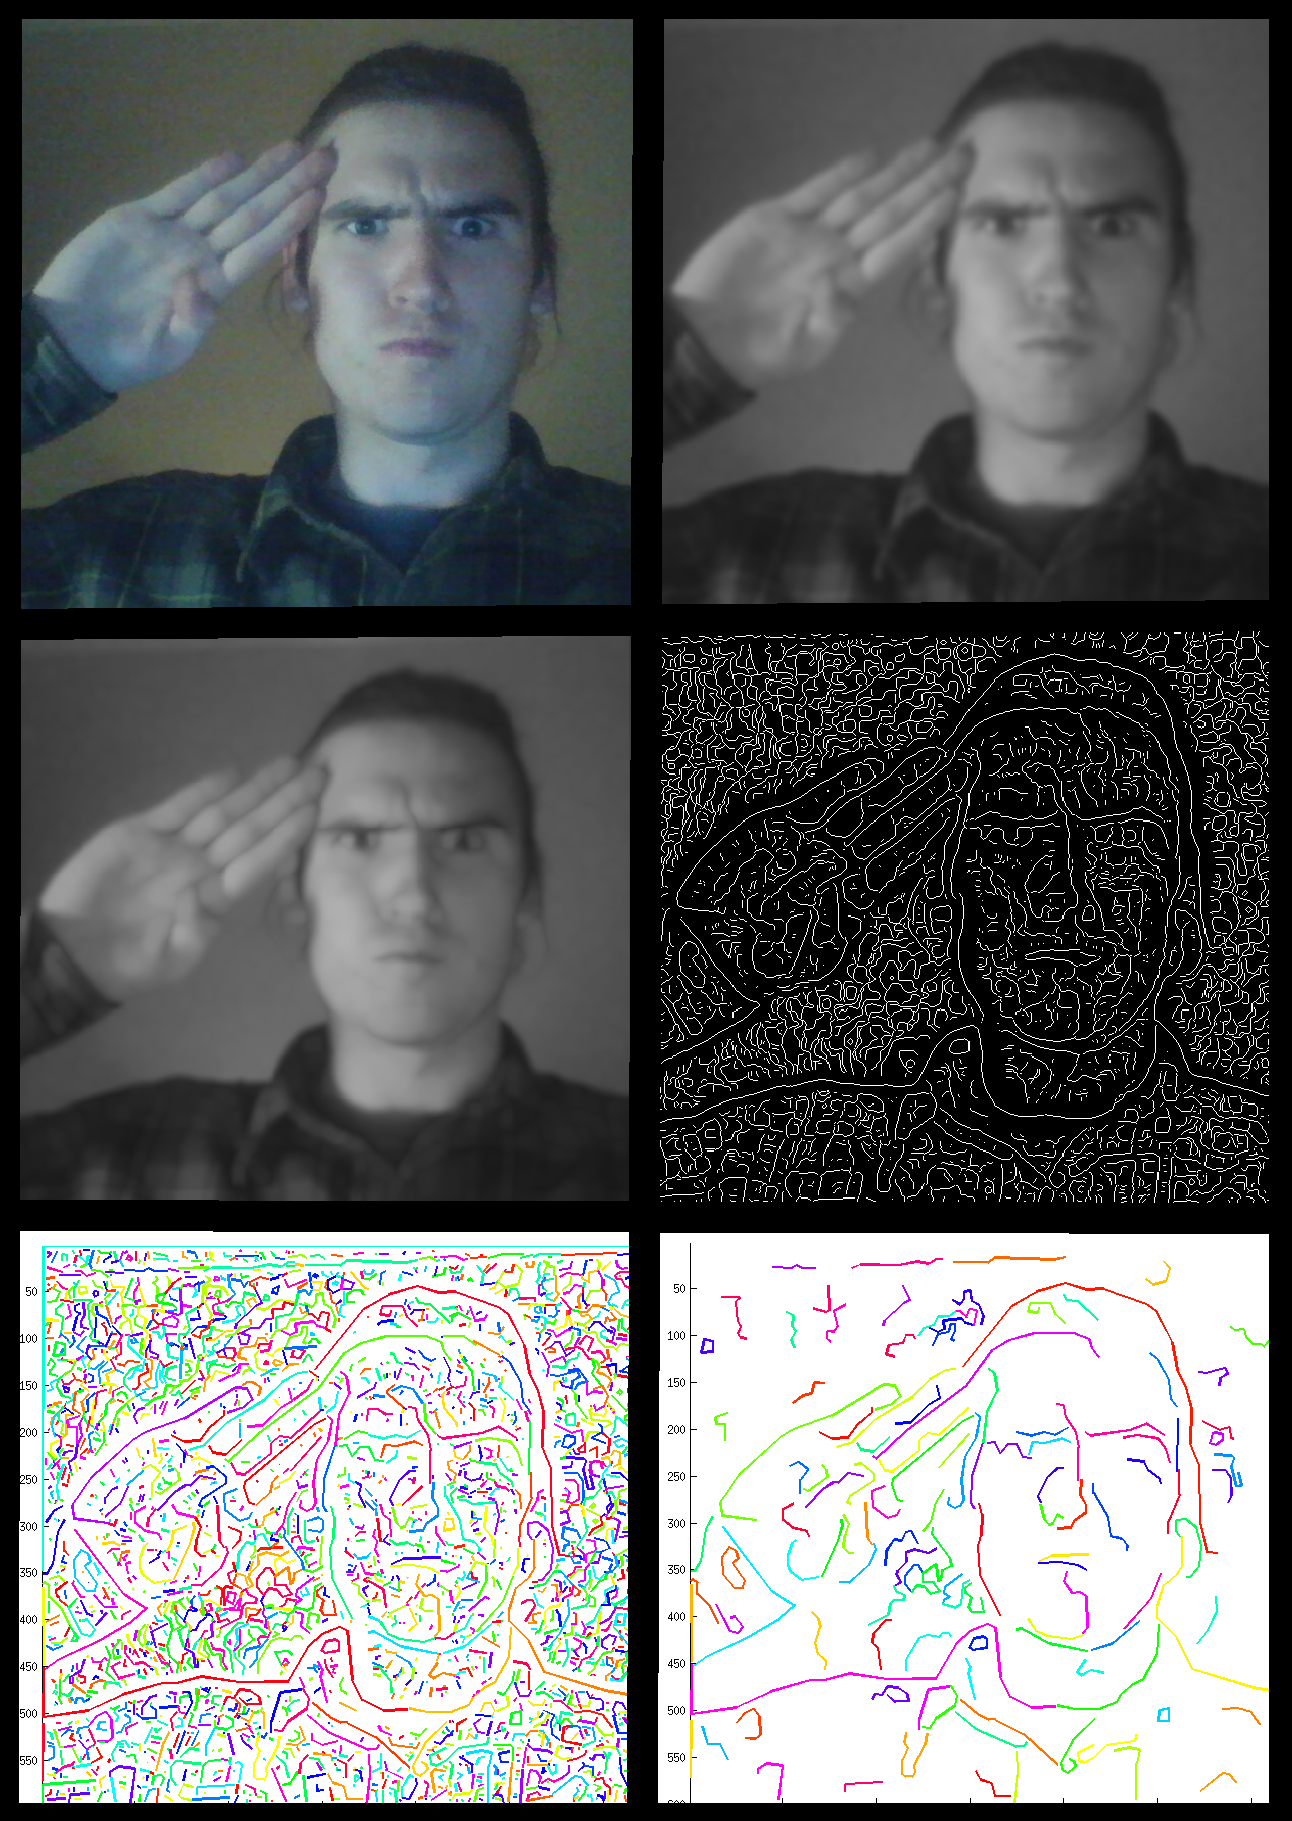
\includegraphics[width=0.9\textwidth]{figures/systemDesign/demo.png}
\caption[Image filtering process] A series of images demonstrating the steps in the image filtering process. From top left to bottom right; 1. Initial Image 2. Gaussian filter 3. Image dilation 4. Canny edge detector 5. Linear edge approximation 6. Edge culling {
\label{fig:demo}}
\end{figure}
